\section{Camera calibration}

Camera calibration is the process of estimating the parameters of a vision system.
Three types of calibration parameters exist: distortion, intrinsics and extrinsics.

\subsection[Distortion]{Distortion~\cite{calib-dist}}

\subsubsection{What is distortion}

A camera lens can introduce two types of distortion: radial and tangential.
Radial distortion makes straight lines appear curved in the image, while tangential distortion can make some image parts look closer than they are.
Figure~\ref{fig:distortion} provides a graphical example of both distortion problems.

\begin{figure}
	\centerline{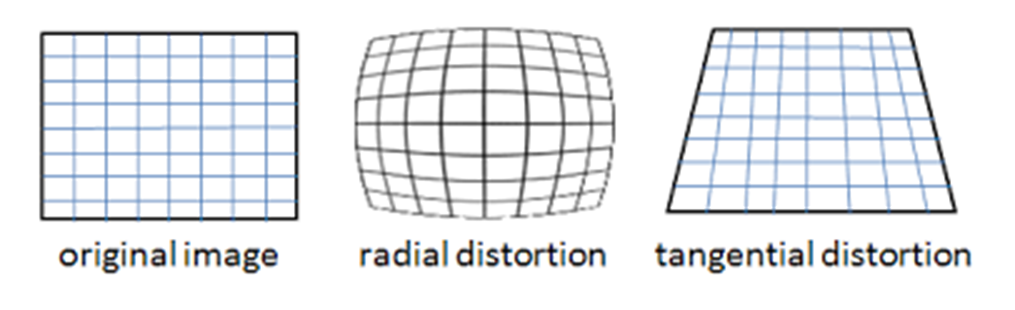
\includegraphics[width=0.6\textwidth]{images/distortion.png}}
	\caption{\centering How radial and tangential distortion affect an image}
	\label{fig:distortion}
\end{figure}

\subsubsection{Mathematical definition}

Given an undistorted point $P=\colvectwo{x}{y}$ (at distance $r$ from the center of the image), a radial distortion will transform it into
\begin{equation}
	P_{dist} = \left( 1 + k_1{\cdot}r^2 + k_2{\cdot}r^4 + k_3{\cdot}r^6 \right) \cdot \colvectwo{x}{y}
\end{equation}
while a tangential distortion would transform it into
\begin{equation}
	P_{dist} = \colvectwo{x+\left[ 2p_1xy + p_2{\cdot}\left( r^2+2x^2 \right) \right]}{y+\left[ 2p_2xy + p_1{\cdot}\left( r^2+2y^2 \right) \right]}
\end{equation}
As such, the full distortion can be described with the vector $\rowvecfive{k_1}{k_2}{p_1}{p_2}{k_3}$

\subsubsection{How to calibrate the parameters}

The estimation of the distortion parameters (among with other parameters) can be computed using \texttt{OpenCV}'s \texttt{calibrateCamera} function.
It requires data extracted from multiple calibration frames, each one with a set of coplanar points.
Each frame must provide the list of pixel coordinates of the points detected in the image.
On top of that, each point must be labeled with a coordinate system local to the plane where the points lay: an example can be a row/column index for a grid-like pattern.

Common calibration patterns are dots (figure~\ref{fig:calibration-planes}.a) or the corners of a chessboard (figure~\ref{fig:calibration-planes}.b).
Often, to help the detection of the chessboard corners, ArUco~\cite{aruco} markers are added in the white cells (figure~\ref{fig:calibration-planes}.c).
This combination of \textbf{ch}essboard and \textbf{ArUco} markers is called \textbf{ChArUco}.

\begin{figure}
	\centering
	\minipage{0.27\textwidth}
	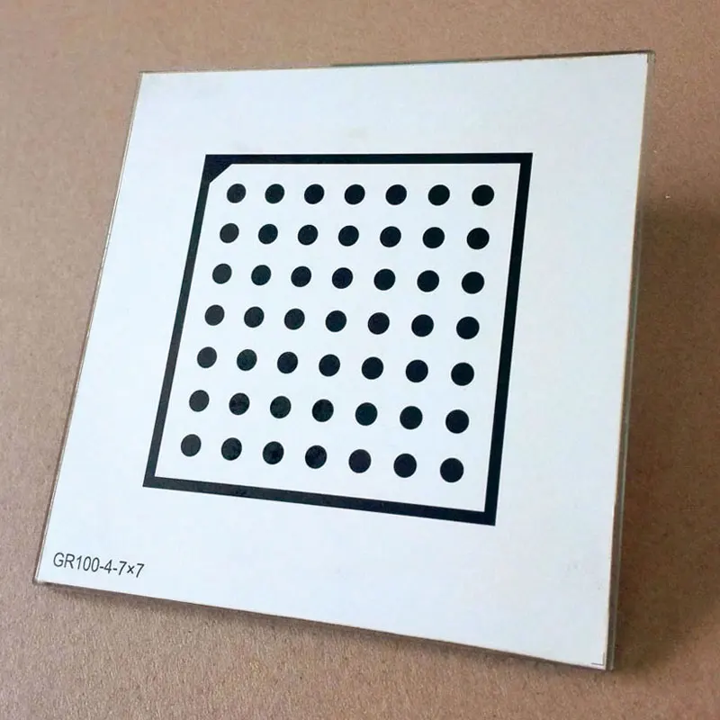
\includegraphics[width=\linewidth]{images/calib-dots.png}
	\caption*{(a)}
	\endminipage\hfill
	\minipage{0.35\textwidth}
	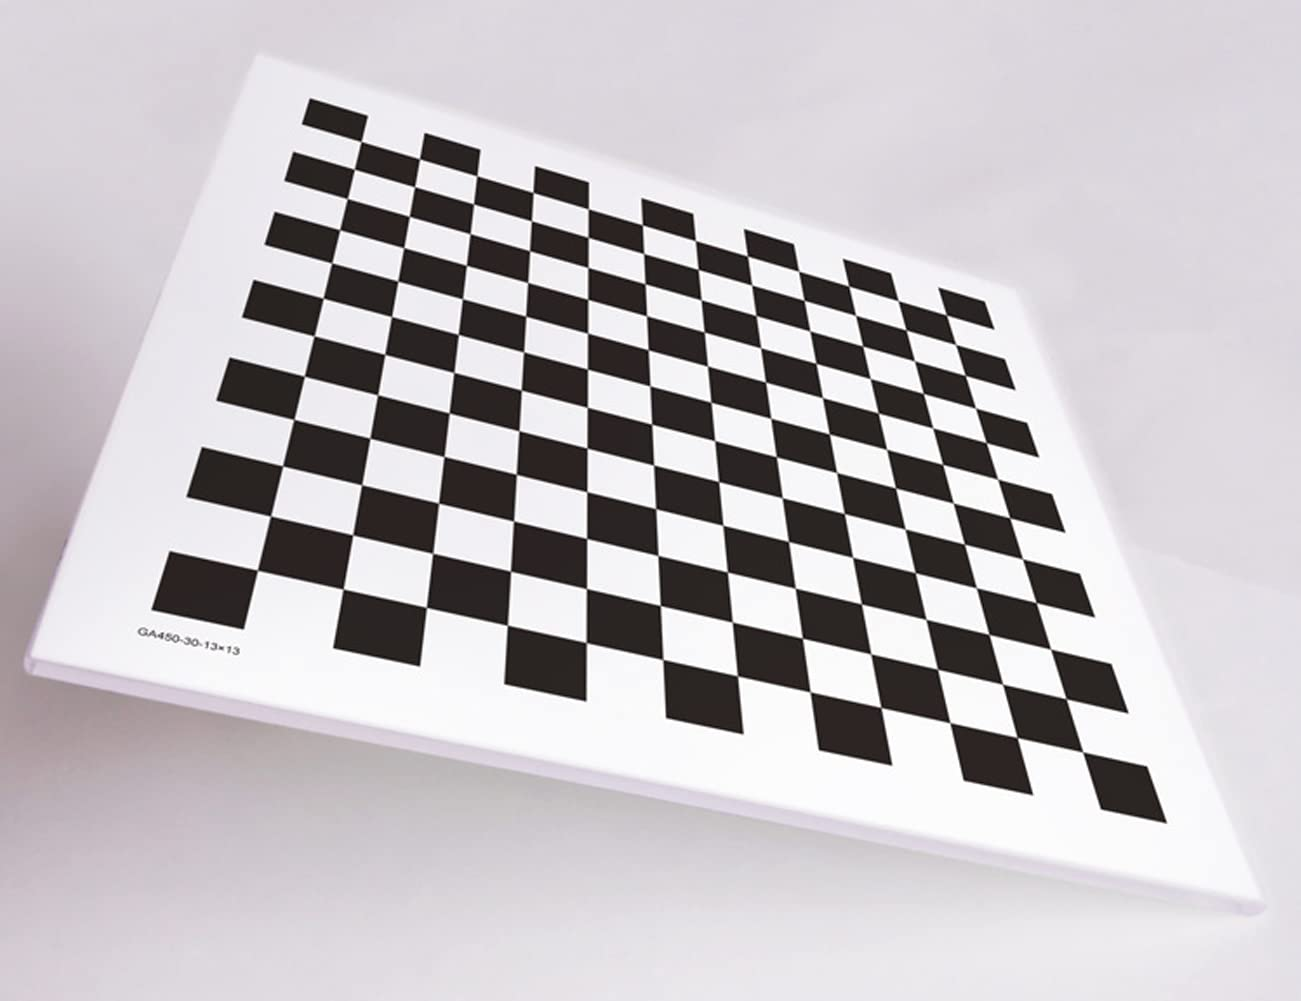
\includegraphics[width=\linewidth]{images/calib-chessb.jpg}
	\caption*{(b)}
	\endminipage\hfill
	\minipage{0.36\textwidth}
	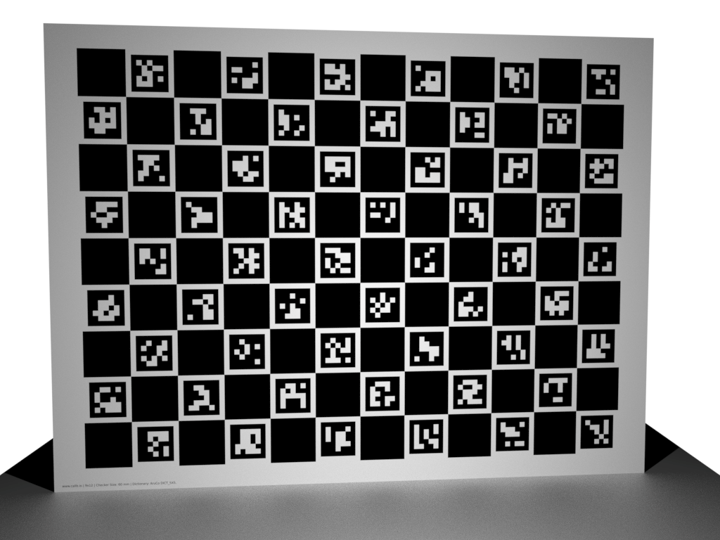
\includegraphics[width=\linewidth]{images/calib-charuco.png}
	\caption*{(c)}
	\endminipage
	\caption{Calibration planes: (a) dots, (b) chessboard, (c) ChArUco.}\label{fig:calibration-planes}
\end{figure}

\subsubsection{How to remove distortion}
Using \texttt{OpenCV}'s \texttt{undistort} function, it is possible to remove the lens distortion.
The result is the image as it would be taken by an ideal camera setup.

\subsection[Intrinsic parameters]{Intrinsic parameters~\cite{calib-intrinsics}}

\subsubsection{What are intrinsic parameters}

The intrinsic parameters describe how the lens and sensor alter the image captured by a single camera.
Using these parameters, it is possible to remove all this distortion, transforming the image into a common frame of reference.
These transforms allow to obtain the same image when two different cameras, with different optics, photograph the same scene.

\subsubsection{Mathematical definition}

Consider a simple scene, with a camera observing a point.
Define a frame of reference centered in the camera.
The point can be described as $R=\rowvecthree{P_x}{P_y}{P_z}^T$.
The camera will project the point onto the image plane, at the homogeneous coordinate $R'=\rowvecthree{P_x'}{P_y'}{1}^T$.
It is possible to show that $P'$ can be written as $P$ transformed by a matrix $K$, called \textbf{intrinsic matrix}: $P' = K{\cdot}P$.

In particular, $K$ is in the form:
\begin{equation}
	K = \begin{bmatrix}
		f_x & s   & x_0 \\
		0   & f_y & y_0 \\
		0   & 0   & 1   \\
	\end{bmatrix}
\end{equation}
where:
\begin{itemize}
	\itemsep 0em
	\item $f_x$ and $f_y$ are the focal lengths in pixels of the optic system. They may differ along the horizontal and vertical direction;
	\item $s$ is the skew, that can be caused by the digitization process;
	\item $x_0$ and $y_0$ are the coordinates of the pixel where the center of projection of the camera stands.
	      % \item $x_0$ and $y_0$ are the horizontal and vertical offset in pixels between the center of projection and the bottom-left corner of the sensor.
\end{itemize}

\subsubsection{How to calibrate the parameters}

The full intrinsic matrix is estimated by the same \texttt{OpenCV} function that evaluates the distortion coefficients.

\subsubsection{How to remove intrinsic parameters}
Using \texttt{OpenCV}'s \texttt{undistort} function, it is possible to remove also the intrinsic parameters.
The result is the image as it would be taken by a camera with $K{=}I_3$.
This enables to compare pixel-wise images captured with different optic and sensor arrangements.

\subsection{Extrinsic parameters}

\subsubsection{What are extrinsic parameters}

The extrinsic parameters describe position and orientation of a camera with respect to a specific frame of reference.
Usually they are not computed when a single camera is present, since it is convenient to assume as frame of reference the position and orientation of the camera.
With multiple cameras, usually one of them is chosen as ``main'', and it acts as the frame of reference for the other cameras.
In this frame of reference it is therefore crucial to understand position and orientation of all the cameras.

Considering camera $A$ as main, the extrinsic parameters of another camera $B$ can be expressed in three different ways:
\begin{itemize}
	\item \textbf{rotation matrix $R$} and \textbf{translation vector $t$}: $R$ describes how to rotate $A$ to be in the same orientation as $B$ (equivalently, how $B$ is rotated in $A$'s frame of reference); $t$ is the versor in $B$'s frame of reference towards the origin (equivalently, $B$ is located in $-Rt$ in the main frame of reference);
	\item \textbf{essential matrix $E$}. Assuming $P_A=\rowvecthree{x_A}{y_A}{1}$ and $P_B=\rowvecthree{x_B}{y_B}{1}$ are the \textit{undistorted} projections of a point $P$ on the two cameras, $E$ is a matrix such that $P_B \cdot E \cdot P_A^T = 0$. $E$ can also be computed as $E = [t]_{\times}R$, where $[t]_{\times}$ is the matrix representation of the cross product of $t$;
	\item \textbf{fundamental matrix $F$}: the definition is the same as $E$'s, but using the points with $K$ still applied (only the distortion has to be removed). If the two cameras have intrinsic matrices $K_A$ and $K_B$, $F$ can be computed as $F = \left(K_A^{-1}\right)^T \cdot E \cdot K_B^T$.
\end{itemize}

\subsubsection{How to calibrate the parameters}

The extrinsic calibration can be obtained from the same data as the intrinsic calibration, provided that the cameras took a picture of the exact same scene (which likely implies that the pictures must be taken at the exact same time instant).
The calibration points detected on both images can be processed by:
\begin{itemize}
	\itemsep 0em
	\item \texttt{OpenCV}'s \texttt{recoverPose} function to obtain $R$ and $t$;
	\item \texttt{OpenCV}'s \texttt{findEssentialMat} function to obtain $E$;
	\item \texttt{OpenCV}'s \texttt{findFundamentalMat} function to obtain $F$.
\end{itemize}

\subsubsection{How to remove extrinsic parameters}

Non-null extrinsic parameters mean that the two images are fundamentally different, therefore it is not possible to remove these parameters.
Instead, these parameters are essential for reconstructing the 3D scene using stereoscopy.

\subsubsection{Definition up to a scale factor}

If everything (objects in the picture, distances between objects and pixel size and focal lenght of the cameras) is scaled by a factor $k$, then the resulting images do not change.
For this reason, the extrinsic parameters can only be defined up to a scale factor.
Most importantly, this affects $t$: it cannot be the vector of the displacement, since the distance is unknown, but it is only the versor of the direction of the displacement.

This makes the reconstruction (stereoscopy) use an arbitrary unit of measurement, which corresponds to the distance between the cameras.
This must be taken into account particularly if there are more than 2 cameras: each camera will have a different distance from the main one, thus having different units of measurement.
The problem can be solved by computing the scaling factor between the units such that the reconstructed calibration points have coherent distance between the different camera couples.
To have a realistic measurement unit, it is also possible to impose this scaling factor in a way that the distance between the reconstructed points is coherent with the real one.
